\section{Android Apps}\label{sec:sota_apps}
In this section we look at the state of the art within streaming synchronized music between different mobile devices.

The apps which is estimated to be a part of the state of the art is the following:
\begin{itemize}
    \item SoundSeeder
    \item AmpMe
    \item Chorus
\end{itemize}

These apps are found by search on sources like Google, YouTube, App Store, and Google Play Store and from recommendations on forums. 
Another criteria was that the app is not depreciated or abandoned by its developers.
The way to estimate this is by looking at the last update date on Google Play Store and App Store.
For instance if an app have not been updated since 2013 and do not support new devices, it is probably abandoned.

To clarify, Google Play Store and App Store are the official place to install or buy apps for Android and iOS devices respectively.

\subsection{SoundSeeder}
SoundSeeder\footnote{http://soundseeder.com} is an app made by JekApps. 
It is compatible with Android 4.1 and above, for older versions of Android (2.2 -- 4.0),
another app called SoundSeeder Speaker can be used as speaker, but not to play the music.
SoundSeeder also provides a Java application for compatibility with other platforms e.g. Windows, macOS and Linux.
JekApps do not support iOS and Windows Phone\cite{soundseeder_ios}.

The app consists of a top menu and a burger menu at he left side, as seen on \cref{fig:soundseeder_screenshot}.
There the user can choose the different playback possibilities and switch to speaker mode.
The main view of the app is a music player, where the music can be controlled as any other music player. 
To play music to other devices, press the ``add music button'' in the top menu, choose the source of the music and choose the preferred music, and press play. 

To connect to a playing device, select the speaker mode from the side menu and if it finds the device, it connects automatically.
It took a bit of time before the speaker device found the playing device, which can confuse and make the user think he has to connect manually with an IP. 

The process of joining (when the devices are given the time of finding each other) is rather simple.
In regard to the user interface, it is quite clotted with features and menus, which can make the app hard to navigate,
and to know what feature is required to go to the next step of a task.
The design of the app is old and not and not very pretty.

SoundSeeder streams music via Wi-Fi or the build--in Android hotspot\cite{soundseether_faq}, 
which means that all phones have to be on the same network.
In regard to the music source, it can be Google Music, YouTube (via semperVidLinks app), online radio stations, UPnP and DLNA devices, and local media.
SoundSeeder also supports to stream from an external source, e.g. a microphone or AUX device. 
The supported media format is depended on the used device and Android version.\cite{soundseether_faq}

SoundSeeder is free to install but the free version is only possible to use with two devices connected as speakers for up to 15 minutes at the time and it do also contains banner adds.
The full app costs 39.90 DKK. 

\begin{figure}[h!]
    \centering
    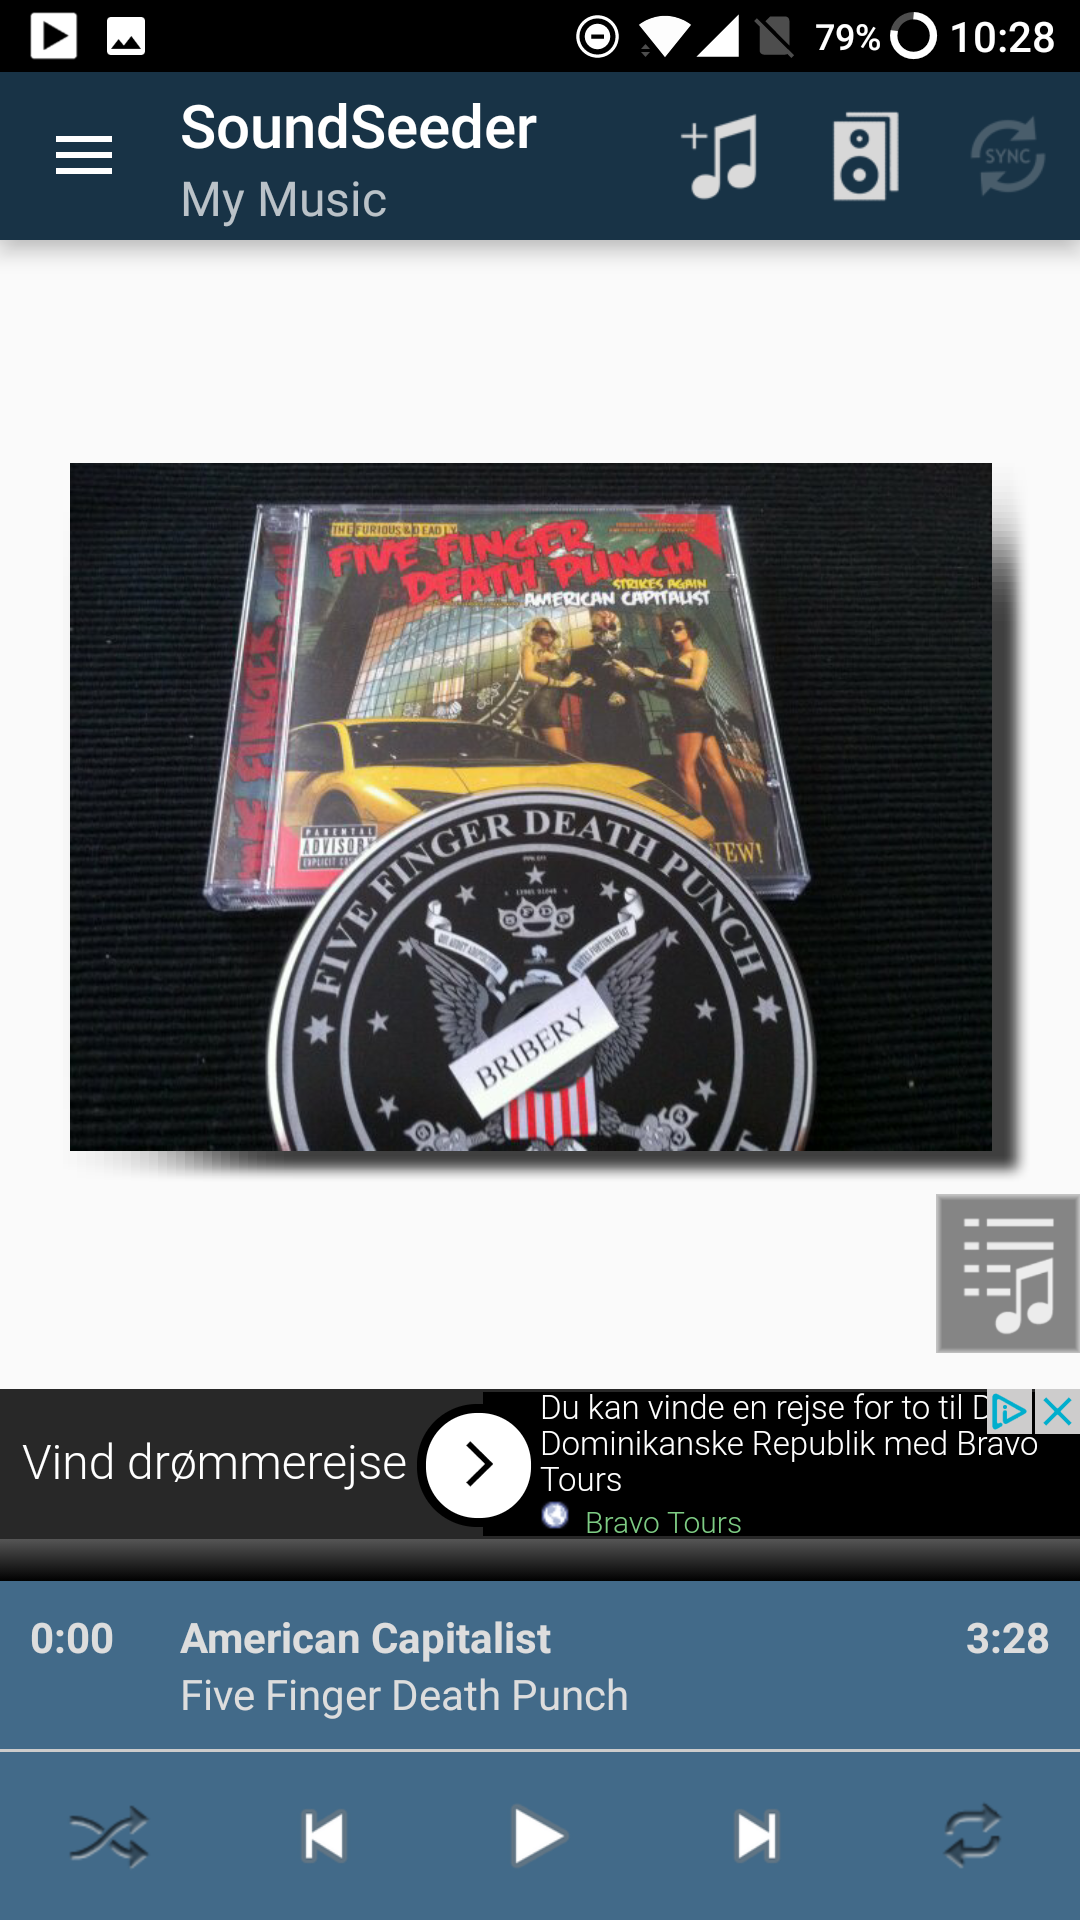
\includegraphics[width=0.3\textwidth]{img/soundseeder.png}
    \caption{A screenshot of SoundSeeder when the app is opened.}
    \label{fig:soundseeder_screenshot}
\end{figure}

\iffalse
3.9 stars on Google Play
Functionality / How good it works
11. november 2016 https://play.google.com/store/apps/details?id=com.kattwinkel.android.soundseeder.player
For Android > 4.1 and Java based devices (RPI, Linux, Windows, macOS etc.), no plans for iOS and Windows Phone http://soundseeder.com/support/topic/ios-and-windows-support-soon/
Google Music, YouTube (via semperVidLinks app), online radiostations, 
Steam music via Wi-Fi or portable hotspot, UPnP/DLNA browser, mp3, mp4, m4a, aac, 3gp, ogg, flac (depends on your device / android version)
Free version: two speaksers for up to 15 min as often you want, it contains banner adds. Priced version: 39,90 DKK
Sync settings: ?
\fi

\subsection{AmpMe}
The second app is AmpMe\footnote{http://www.ampme.com}, made by Amp Me Inc., which is another app to synchronize music between devices.
It supports Android 4.1 or newer and iOS 9.0 or newer.

In AmpMe the music player with the connected devices is called ``a party''.
When AmpMe is opened, it either displays the nearby parties or encourage you to create your own. 
If a party if found, you can join it and have your device work as a speaker.
If no party is found, or you want to create your own, you can choose to start it by choosing between Spotify, 
YouTube, your own music library, or SoundCloud as music source, as shown on \cref{fig:ampme_screenshot}. 
Then when the source type and music is chosen, a player appears with the music playing.

It is very intuitive to join a party, or host one yourself and play music.
Furthermore the interface is modern, minimalistic, and pleasant to use and look at. 

To be able to stream music between devices, AmpMe require internet, in the form of WiFi or mobile data.
This means that the connected devices can be on WiFi, mobile data or another network, as long there is Internet access. 
As for the music source, AmpMe supports Spotify, SoundCloud, YouTube and local media.
AmpMe is free to use in both Google Play and App Store.\cite{amp_faq}\cite{amp_play}\cite{amp_itunes}

\begin{figure}[h!]
    \centering
    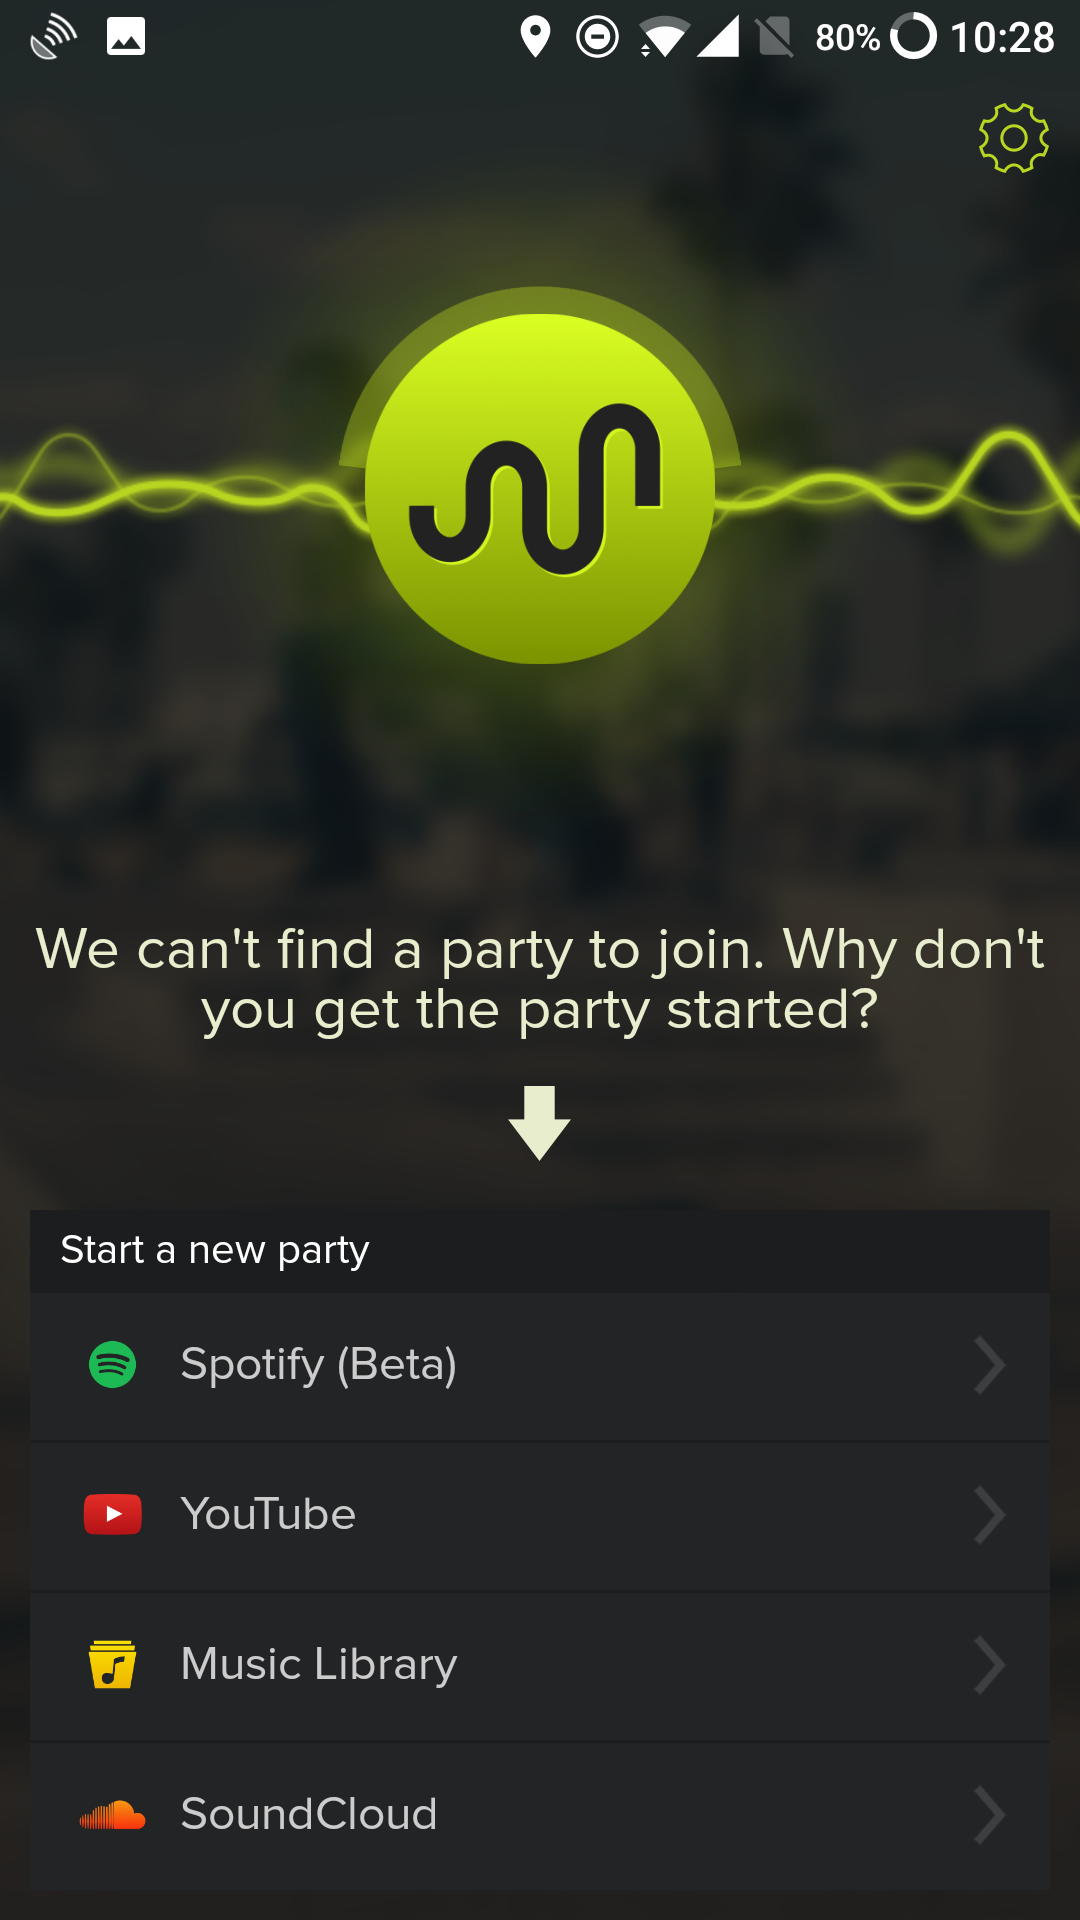
\includegraphics[width=0.3\textwidth]{img/ampme.png}
    \caption{A screenshot of AmpMe when the app is opened.}
    \label{fig:ampme_screenshot}
\end{figure}

\iffalse
By Amp Me Inc.
4.2 stars on Google Play, current version, 3.5 stars, all versions 4 stars on App Store
Functionality / How good it works
30. januar 2017 (Android), Feb 01, 2017 (iOS)
Android and iOS
Spotify, SoundCloud, YouTube and your local music library
Require internet, WiFi/Mobile data
Free
Resync button, syncs upon connection
\fi

\subsection{Chorus}
The final app is called Chorus\footnote{https://play.google.com/store/apps/details?id=com.avrapps.chorus} and is made by AVR APPS.
Is supports Android 4.0 or newer, they state to have an iOS app, but the App Store page returns that the app is not available in our region,
when open in iTunes\footnote{https://itunes.apple.com/app/chorus/id894014439}.

When the app is opened, it basically looks like a regular music player, as seen on \cref{fig:chorus_screenshot}.
Music is added by pressing the small plus sign in the right bottom corner. 
When that music is added, Chorus streams the music to connected devices. 
To join another user playing music, you press the menu button in the right top corner, and press join.
Here a menu pops up with devices playing on the network, and if you selects the device shown, it connects and starts playing.
The first attempt of connecting to the playing device was unsuccessful, it just kept on loading, after a restart of the app it worked.

It is intuitive to use the app, it is very minimalistic hence easy to navigate.
The design is a bit old but its simplicity makes up for it.

To share music between devices, WiFi or mobile hotspot is required,
which means that all devices have to be on the same network.
Chorus only supports playback of local media, so the music have to be locally on the device.
The app is free to download and use without any adds.\cite{chrous_play} 

\begin{figure}[h!]
    \centering
    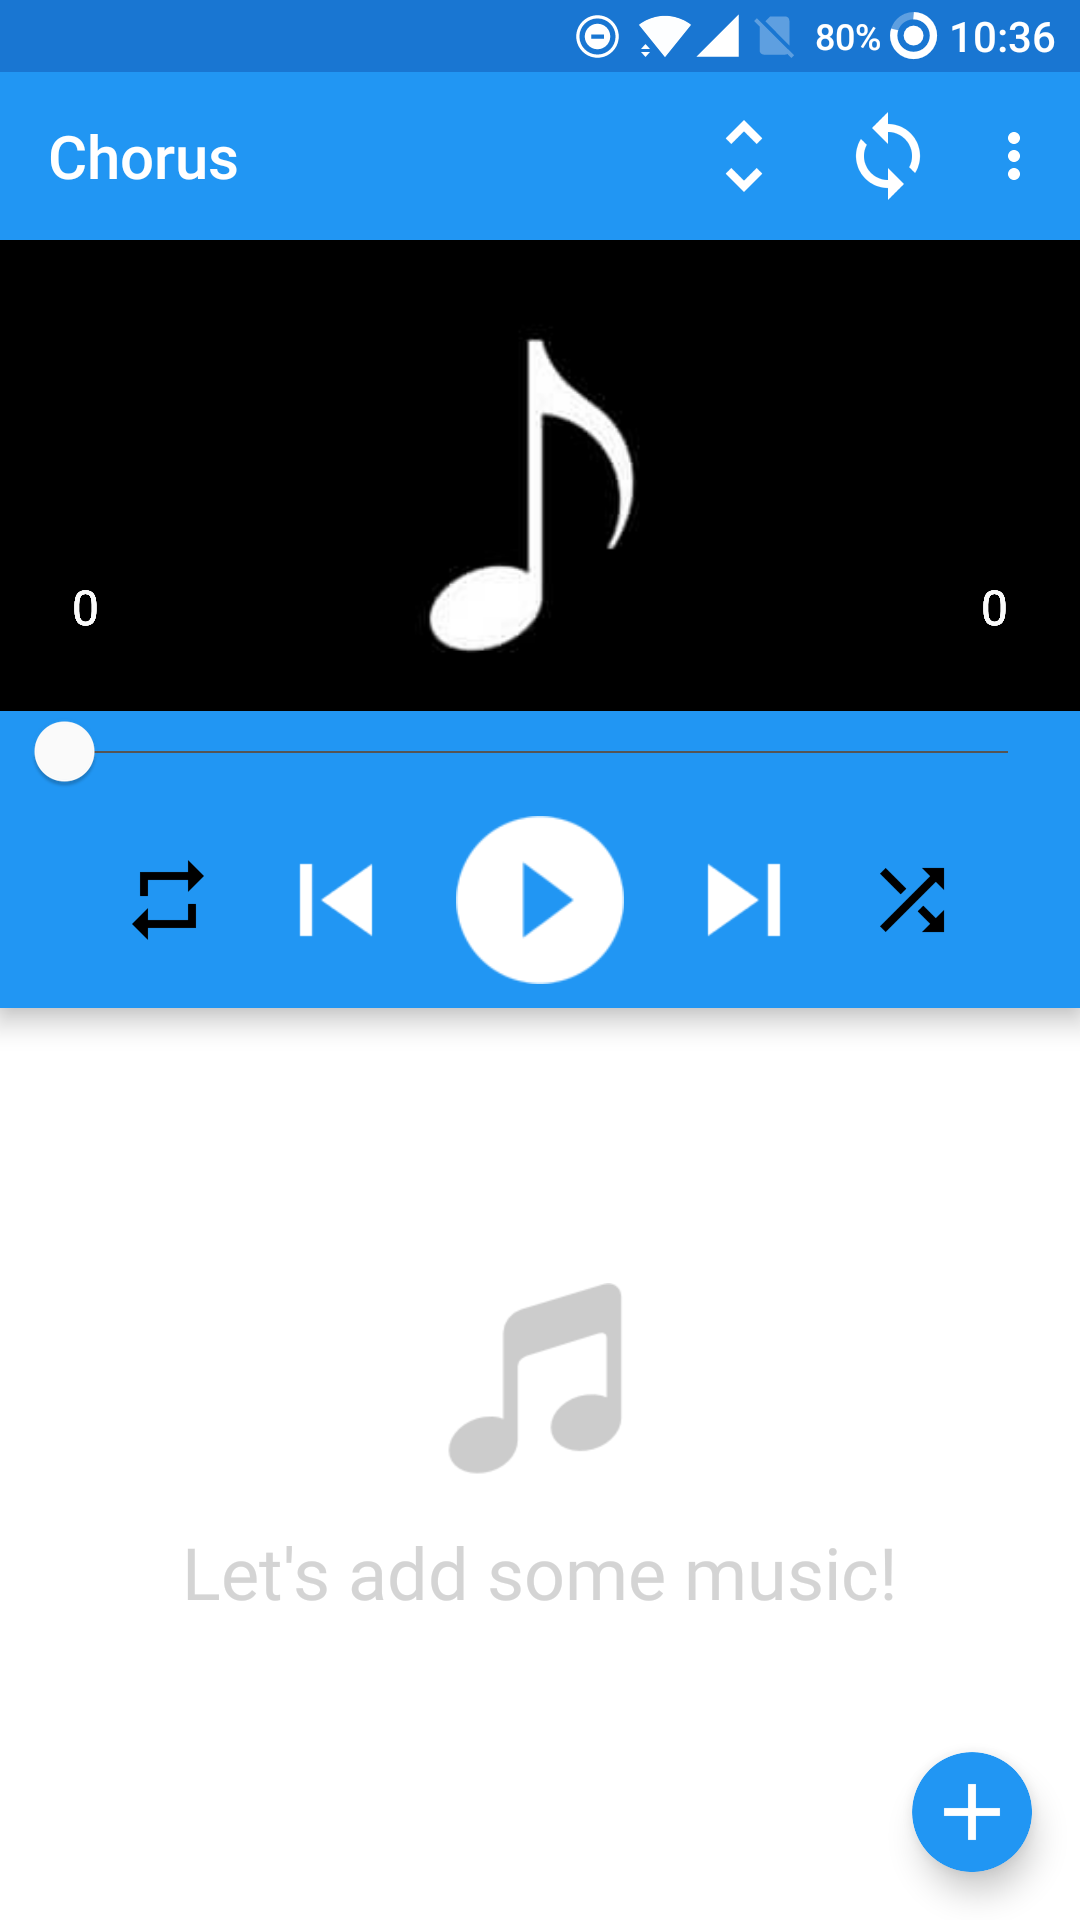
\includegraphics[width=0.3\textwidth]{img/chorus.png}
    \caption{A screenshot of Chorus when the app is opened.}
    \label{fig:chorus_screenshot}
\end{figure}

\iffalse
By AVR APPS 
3.3 stars on Google Play
Functionality / How good it works
11. maj 2015
Android 4.0, iOS
Local media?
Mobile hotspot or WiFi
Free
Manual/automatic sync
\fi
\subsection{Comparison}
\iffalse
        Func1 FUnc2 
App1
App2
App3
\fi

\begin{tabular}{l|l|l|p{2.5cm}|p{2.5cm}|p{2.5cm}|p{2.5cm}|}
                & Rating    & Last update   & Supported devices & Media source & Connectivity & Pricing  \\
    \toprule
    SoundSeeder & 3.9       & 11/11 2016    & Android 4.1 and above, Java devices & Google Music, YouTube, online radio, local media & asdf & Free (limited) or 39.90 DKK \\
\end{tabular}

